\documentclass[11pt]{article}
\usepackage{epsfig,psfrag}
\usepackage{amsmath}

\setlength{\textwidth}{6.2in}
\setlength{\oddsidemargin}{0.3in}
\setlength{\evensidemargin}{0in}
\setlength{\textheight}{8.7in}
\setlength{\voffset}{-.7in}
\setlength{\headsep}{26pt}
\setlength{\parindent}{10pt}
\begin{document}


% a few handy macros

\newcommand\matlab{{\sc matlab}}
\newcommand{\goto}{\rightarrow}
\newcommand{\bigo}{{\mathcal O}}
\newcommand{\half}{\frac{1}{2}}
%\newcommand\implies{\quad\Longrightarrow\quad}
\newcommand\reals{{{\rm l} \kern -.15em {\rm R} }}
\newcommand\complex{{\raisebox{.043ex}{\rule{0.07em}{1.56ex}} \hskip -.35em {\rm C}}}


% macros for matrices/vectors:

% matrix environment for vectors or matrices where elements are centered
\newenvironment{mat}{\left[\begin{array}{ccccccccccccccc}}{\end{array}\right]}
\newcommand\bcm{\begin{mat}}
\newcommand\ecm{\end{mat}}

% matrix environment for vectors or matrices where elements are right justifvied
\newenvironment{rmat}{\left[\begin{array}{rrrrrrrrrrrrr}}{\end{array}\right]}
\newcommand\brm{\begin{rmat}}
\newcommand\erm{\end{rmat}}

% for left brace and a set of choices
\newenvironment{choices}{\left\{ \begin{array}{ll}}{\end{array}\right.}
\newcommand\when{&\text{if~}}
\newcommand\otherwise{&\text{otherwise}}
% sample usage:
%  \delta_{ij} = \begin{choices} 1 \when i=j, \\ 0 \otherwise \end{choices}


% for labeling and referencing equations:
\newcommand{\eql}{\begin{equation}\label}
\newcommand{\eqn}[1]{(\ref{#1})}
% can then do
%  \eql{eqnlabel}
%  ...
%  \end{equation}
% and refer to it as equation \eqn{eqnlabel}.  


% some useful macros for finite difference methods:
\newcommand\unp{U^{n+1}}
\newcommand\unm{U^{n-1}}

% for chemical reactions:
\newcommand{\react}[1]{\stackrel{K_{#1}}{\rightarrow}}
\newcommand{\reactb}[2]{\stackrel{K_{#1}}{~\stackrel{\rightleftharpoons}
   {\scriptstyle K_{#2}}}~}

  % input some useful macros

% Macros for exercises:

\newcommand{\exernum}{0.0} % will be set to current Exercise number

% Headers:

\newcommand{\exercise}[2][\null]{\vskip 15pt \noindent%
     {\large \bf Exercise #2}~ {\it #1}%
     \nopagebreak\vskip 5pt \nopagebreak%
     \renewcommand{\exernum}{#2} \setcounter{equation}{0}%
     \addcontentsline{toc}{subsection}{Exercise #2 \hskip 5pt #1}}
     % \exercise has optional first argument -- short descriptor
     % the exercise number is stored in \exernum for use in labeling equations

\newcommand{\chapexercises}[1]{%
     \cleardoublepage
     \centerline{\LARGE\bf Chapter #1 Exercises}
     \vskip .5cm
     \noindent
     From: {\it Finite Difference Methods for Ordinary and Partial 
     Differential Equations}\\  by R.~J.~LeVeque, SIAM, 2007.~~~
     {\tt http://www.amath.washington.edu/$\sim$rjl/fdmbook}
     \vskip .5cm
     \addcontentsline{toc}{section}{Chapter #1}
     }

% Parts:

% set enumerate to give parts a, b, c, ...  rather than numbers 1, 2, 3...
\renewcommand{\theenumi}{\alph{enumi}}
\renewcommand{\labelenumi}{(\theenumi)}

% set second level enumerate to give parts i, ii, iii, iv, etc.
\renewcommand{\theenumii}{\roman{enumii}}
\renewcommand{\labelenumii}{(\theenumii)}

% Equations:

% label equations starting with E for exercise, then exernum, then a,b,c etc
\renewcommand{\theequation}{Ex\exernum\alph{equation}}


% commands for labeling and citing equations to add exernum automatically.
%   then set equations using e.g. \eqlex{a} ... \end{equation}
%   and cite as \eqnex{a}
\newcommand{\eqlex}[1]{\begin{equation}\label{\exernum #1}}
\newcommand{\eqnex}[1]{(\ref{\exernum #1})}
       % more macros for exercise formatting


% For exercises,
% set enumerate to give parts a, b, c, ...  rather than numbers 1, 2, 3...
\renewcommand{\theenumi}{\alph{enumi}}
\renewcommand{\labelenumi}{(\theenumi)}

\begin{center}
\sffamily
\huge
Exercises from\\
\vskip 5pt
{\bf Finite Difference Methods for Ordinary and Partial 
Differential Equations}\\  
\LARGE
\vskip 5pt
by Randall J.\ LeVeque\\
SIAM, Philadelphia, 2007\\
\vskip 5pt
\large
{\tt http://www.amath.washington.edu/$\sim$rjl/fdmbook}
\vskip 5pt
Under construction --- more to appear.
\end{center}

\vskip 15pt
{\small
\tableofcontents
}

\chapexercises{1}

\exercise[(derivation of finite difference formula)]{1.1}

Determine the interpolating polynomial $p(x)$ discussed in Example~1.3
and verify that evaluation $p'(\bar x)$ gives equation (1.11).



\exercise[(use of {\tt fdstencil})]{1.2}

\begin{enumerate}
\item
Use the method of undetermined coefficients to set up the $5\times 5$
Vandermonde system that would determine a fourth-order accurate
finite difference approximation to $u''(x)$ based on 5 equally spaced
points,
\[
u''(x) = c_{-2} u(x-2h) + c_{-1} u(x-h) + c_0u(x) + c_1u(x+h) +
c_2u(x+2h) + O(h^4).
\]

\item 
Compute the coefficients using the 
\matlab\ code {\tt fdstencil.m} available from the website, and check that
they satisfy the system you determined in part (a).

\item
Test this finite difference formula to approximate $u''(1)$ for 
$u(x) = \sin(2x)$ with values of $h$ from the array 
{\tt hvals = logspace(-1, -4, 13)}.
Make a
table of the error vs.\ $h$ for several values of $h$ and compare against
the predicted error from the leading term of the expression printed by
{\tt fdstencil}. 
You may want to look at the m-file {\tt chap1example1.m} for
guidance on how to make such a table.

Also produce a log-log plot of the absolute value of the error vs.~$h$.  

You should observe the predicted accuracy for larger values of $h$.  For
smaller values, numerical cancellation in computing the linear combination
of $u$ values impacts the accuracy observed.
\end{enumerate}


\chapexercises{2}

\exercise[(inverse matrix and Green's functions)]{2.1}

\begin{enumerate} 
\item Write out the $5\times 5$
matrix $A$ from (2.43) for the boundary value problem
$u''(x)=f(x)$ with $u(0)=u(1)=0$ for  $h = 0.25$.

\item Write out the $5\times 5$
inverse matrix $A^{-1}$ explicitly for this problem.

\item
If $f(x)=x$, determine the discrete approximation to the solution of the
boundary value problem on this grid and sketch this solution and the five
Green's functions whose sum gives this solution.

\end{enumerate} 


\exercise[(Green's function with Neumann boundary conditions)]{2.2}

\begin{enumerate} 
\item
Determine the Green's functions for the two-point boundary
value problem $u''(x) = f(x)$ on $0<x<1$ with a Neumann boundary condition
at $x=0$ and a Dirichlet condition at $x=1$, i.e, find the function
$G(x,\bar x)$ solving
\[
u''(x) = \delta(x-\bar x), \quad u'(0)=0, \quad u(1)=0
\]
and the functions $G_0(x)$ solving
\[
u''(x) = 0, \quad u'(0)=1, \quad u(1)=0
\]
and $G_1(x)$ solving
\[
u''(x) = 0, \quad u'(0)=0, \quad u(1)=1.
\]

\item 
Using this as guidance, find the general formulas for the elements of the
inverse of the matrix in equation (2.54).  Write out the $5\times 5$ matrices
$A$ and $A^{-1}$ for the case $h=0.25$.
\end{enumerate} 


\exercise[(solvability condition for Neumann problem)]{2.3}

Determine the null space of the matrix $A^T$, where $A$ is given in
equation (2.58), and verify that the condition (2.62) must hold for the
linear system to have solutions.




\exercise[(boundary conditions in {\tt bvp} codes)]{2.4}

\begin{enumerate}

\item Modify the m-file {\tt bvp2.m}
so that it implements a Dirichlet boundary condition at
$x=a$ and a Neumann condition at $x=b$ and test the modified program.

\item Make the same modification to the m-file {\tt bvp4.m}, which
implements a fourth order accurate method.  Again test the modified program.

\end{enumerate} 


\exercise[(accuracy on nonuniform grids)]{2.5}

In Example 1.4 a 3-point approximation to $u''(x_i)$ is determined based on
$u(x_{i-1}),~ u(x_i)$, and $u(x_{i+1})$ (by translating from $x_1$, $x_2$,
$x_3$ to general $x_{i-1}$, $x_i$, and $x_{i+1}$).  
It is also determined that the truncation
error of this approximation is $\frac 1 3 (h_{i-1}-h_i) u'''(x_i) + O(h^2)$,
where $h_{i-1} = x_i-x_{i-1}$ and $h_i = x_{i+1}-x_i$, so the approximation is
only first order accurate in $h$ if $h_{i-1}$ and $h_i$ are  $O(h)$ but
$h_{i-1}\neq h_i$.  

The program {\tt bvp2.m} is based on using 
this approximation at each grid point, as described in Example 2.3.  
Hence on a nonuniform grid the local
truncation error is $O(h)$ at each point, where $h$ is some measure of the
grid spacing (e.g., the average spacing on the grid).  If we
assume the method is stable, then we expect the global error to be $O(h)$ as
well as we refine the grid.

\begin{enumerate}
\item
However, if you run {\tt bvp2.m} you should observe second-order
accuracy, at least provided you take a smoothly varying grid (e.g., set
{\tt gridchoice = 'rtlayer'} in {\tt bvp2.m}).  Verify this.

\item
Suppose that the grid is defined by $x_i = X(z_i)$ where $z_i = ih$ for
$i=0,~1,~\ldots,~m+1$ with $h=1/(m+1)$
is a uniform grid and $X(z)$ is some smooth mapping
of the interval $[0,1]$ to the interval $[a,b]$.  Show that if $X(z)$ is
smooth enough, then the local truncation error is in fact $O(h^2)$.
Hint: $x_i-x_{i-1} \approx hX'(x_i)$.

\item
What average order of accuracy is observed on a random grid?  To test this,
set {\tt gridchoice = 'random'} in {\tt bvp2.m} and increase the number of
tests done, e.g., by setting {\tt mvals = round(logspace(1,3,50));}
to do 50 tests for values of $m$ between 10 and 1000.
\end{enumerate}



\exercise[(ill-posed boundary value problem)]{2.6}

Consider the following linear boundary value problem
with Dirichlet boundary conditions:
\begin{equation*} 
\begin{split}
&u''(x) +  u(x) = 0 \quad \text{for $a< x< b$}\\
&u(a)=\alpha,\quad u(b)=\beta.
\end{split}
\end{equation*}
Note that this equation arises from a linearized pendulum, for example.

\begin{enumerate} 
\item
Modify the m-file {\tt bvp2.m} to solve this problem.  Test your modified
routine on the problem with
\[
a = 0, \quad b = 1, \quad \alpha = 2, \quad \beta = 3.
\]
Determine the exact solution for comparison.

\item 
Let $a=0$ and $b=\pi$. 
For what values of $\alpha$ and $\beta$  does this boundary value problem
have solutions?
Sketch a family of solutions in a case where there are infinitely many
solutions.

\item Solve the problem with 
\[
a = 0, \quad b = \pi, \quad \alpha = 1, \quad \beta = -1.
\]
using your modified {\tt bvp2.m}.  Which solution to the boundary value
problem does this appear to converge to as $h\goto 0$?  Change the boundary
value at $b=\pi$ to $\beta = 1$.  Now how does the numerical solution behave
as $h\goto 0$?

\item You might expect the linear system in part (c) to be singular since
the boundary value problem is not well posed.  It is not, because of
discretization error.  Compute the eigenvalues of the matrix $A$ for this
problem and show that an eigenvalue approaches 0 as $h\goto 0$.
Also show that $\|A^{-1}\|_2$ blows up as $h\goto 0$ so that the
discretization is unstable.

\end{enumerate} 


\exercise[(nonlinear pendulum)]{2.7}

\begin{enumerate} 

\item Write a program to solve the boundary value problem for the
nonlinear pendulum as discussed in the text.  See if you can find yet
another solution for the boundary conditions illustrated in Figures 2.4
and 2.5.

\item Find a numerical solution to this BVP with the same
general behavior as seen in Figure 2.5 for the case of a longer time
interval, say $T=20$, again with $\alpha=\beta=0.7$.  Try larger values of
$T$.  What does $\max_i \theta_i$ approach as $T$ is increased?  Note that
for large $T$ this solution  exhibits ``boundary layers''.

\end{enumerate} 


\chapexercises{3}

\exercise[(code for Poisson problem)]{3.1}

The \matlab\ script {\tt poisson.m} solves the Poisson problem on a square
$m\times m$ grid with $\Delta x = \Delta y = h$, using the 5-point
Laplacian.  It is set up to solve a test problem for which the exact
solution is $u(x,y) = \exp(x+y/2)$, using Dirichlet boundary conditions and
the right hand side $f(x,y) = 1.25 \exp(x+y/2)$.

\begin{enumerate} 
\item Test this script by performing a grid refinement study to verify that
it is second order accurate.

\item Modify the script so that it works on a rectangular domain $[a_x,b_x]
\times [a_y,b_y]$, but still with $\Delta x = \Delta y = h$.  Test your
modified script on a non-square domain.

\item Further modify the code to allow $\Delta x \neq \Delta y$ and test the
modified script.
\end{enumerate} 


\exercise[(9-point Laplacian)]{3.2}

\begin{enumerate}
\item
Show that the 9-point Laplacian (3.17) has the truncation error derived in
Section 3.5.
{\bf Hint:} To simplify the computation, note that the 9-point Laplacian can
be written as the 5-point Laplacian (with known truncation error) plus a
finite difference approximation that models $\frac 1 6 h^2 u_{xxyy} +
O(h^4)$.

\item
Modify the \matlab\ script {\tt poisson.m} to use the
9-point Laplacian (3.17) instead of the 5-point Laplacian, and to solve the
linear system (3.18) where $f_{ij}$ is given by (3.19).  Perform a grid
refinement study to verify that fourth order accuracy is achieved.

\end{enumerate} 




\chapexercises{4}

\exercise[(Convergence of SOR)]{4.1}

The m-file \verb+iter_bvp_Asplit.m+ implements the Jacobi, Gauss-Seidel, and
SOR matrix splitting methods on the linear system arising from the boundary
value problem $u''(x) = f(x)$ in one space dimension.  

\begin{enumerate}
\item Run this program for each method and produce a plot similar to 
Figure~4.2.

\item The convergence behavior of SOR is very sensitive to the choice of
$\omega$ ({\tt omega} in the code).  Try changing from the optimal $\omega$
to $\omega = 1.8$ or 1.95.

\item Let $g(\omega) = \rho(G(\omega))$ be the spectral radius of the
iteration matrix $G$ for a given value of $\omega$.  Write a program to
produce a plot of $g(\omega)$ for $0\leq \omega \leq 2$.

\item From equations (4.22) one might be tempted to try to implement SOR as
\begin{verbatim}
     for iter=1:maxiter
        uGS = (DA - LA) \ (UA*u + rhs);
        u = u + omega * (uGS - u);
        end
\end{verbatim}
where the matrices have been defined as in \verb+iter_bvp_Asplit.m+.
Try this computationally and observe that it does not work well.  Explain
what is wrong with this and derive the correct expression (4.24).

\end{enumerate} 


\exercise[(Forward vs.\ backward Gauss-Seidel)]{4.2}

\begin{enumerate}
\item The Gauss-Seidel method for the discretization of $u''(x) = f(x)$
takes the form (4.5) if we assume we are marching forwards across the grid,
for $i=1,~2,~\ldots,~m$.  We can also define a {\it backwards Gauss-Seidel
method} by setting
\eqlex{a}
u_i^{[k+1]} = \half (u_{i-1}^{[k]} + u_{i+1}^{[k+1]} - h^2 f_i), \qquad
\text{for}~ i = m,~m-1,~m-2,~\ldots,~1.
\end{equation}
Show that this is a matrix splitting method of the type described in
Section~4.2 with $M = D-U$ and $N=L$.

\item Implement this method in \verb+iter_bvp_Asplit.m+ and observe that it
converges at the same rate as forward Gauss-Siedel for this problem.

\item Modify the code so that it solves the boundary value problem
\eqlex{b}
\epsilon u''(x) = au'(x) + f(x),\qquad 0\leq x \leq 1,
\end{equation} 
with $u(0) = 0$ and $u(1) = 0$, where $a\geq 0$ and the $u'(x_i)$ term
is discretized by the one-sided approximation $(U_i - U_{i-1})/h$.
Test both forward and backward Gauss-Seidel for the resulting linear system.
With $a=1$ and $\epsilon = 0.0005$.  You should find that they behave very
differently:

\psfrag{forwardGS}{forward}
\psfrag{backwardGS}{backward}
\hfil\epsfig{file=figs/iter_bvp_advdiff.eps,width=3.5in}\hfil

Explain intuitively why sweeping in one direction works so much better than
in the other.

{\bf Hint:} Note that this equation is the steady equation for an 
advection-diffusion
PDE $u_t(x,t) + au_x(x,t) = \epsilon u_{xx}(x,t) - f(x)$.  
You might consider how the methods behave in the case $\epsilon = 0$.
\end{enumerate} 


\chapexercises{5}

\exercise[(Uniqueness for an ODE)]{5.1}

Prove that the ODE 
\[
u'(t) = \frac 1 {t^2 + u(t)^2}, \quad \mbox{for}~t \geq 1
\]
has a unique solution for all time from any initial value $u(1)=\eta$.




\exercise[(Lipschitz constant for an ODE)]{5.2}

Let $f(u) = \log(u)$.
\begin{enumerate}
\item Determine the best possible Lipschitz constant for this function over
$2\leq u < \infty$.

\item Is $f(u)$ Lipschitz continuous over $0<u<\infty$?

\item Consider the initial value problem
\begin{equation*}
\begin{split}
u'(t) &= \log(u(t)),\\
u(0) &= 2.
\end{split}
\end{equation*}
Explain why we know that this problem has a unique solution for all $t\geq 0$
based on the existence and uniqueness theory described in Section 5.2.1.
(Hint: Argue that $f$ is Lipschitz continuous in  a domain that the
solution never leaves, though the domain is
not symmetric about $\eta=2$ as assumed in the theorem quoted in the book.)
\end{enumerate} 



\exercise[(Lipschitz constant for a system of ODEs)]{5.3}

Consider the system of ODEs
\begin{equation*}
\begin{split}
u_1' &= 3u_1 + 4u_2,\\
u_2' &= 5u_1 - 6u_2.\\
\end{split}
\end{equation*}
Determine the Lipschitz constant for this system in the max-norm
$\|\cdot\|_\infty$ and the 1-norm $\|\cdot\|_1$. (See Appendix A.3.)




\exercise[(Duhamel's principle)]{5.4}

Check that the solution $u(t)$ given by (5.8) satisfies the ODE (5.6) and
initial condition.  Hint: To differentiate the matrix exponential you can
differentiate the Taylor series (D.31) (in Appendix D) term by term.



\exercise[(matrix exponential form of solution)]{5.5}

The initial value problem
\[
v''(t) = -4v(t), \qquad v(0) = v_0,\quad v'(0) = v_0'
\]
has the solution $v(t) = v_0\cos(2t) + \half v_0' \sin(2t)$.  Determine this
solution by rewriting the ODE as a first order system $u' = Au$ so that
$u(t) = e^{At}u(0)$ and then computing the matrix exponential using (D.30)
in Appendix D.




\exercise[(matrix exponential form of solution)]{5.6}

Consider the IVP
\begin{equation*}
\begin{split}
u_1' &= 2u_1,\\
u_2' &= 3u_1 - u_2,
\end{split}
\end{equation*}
with initial conditions specified at time $t=0$.  Solve this problem in two
different ways:

\begin{enumerate}
\item Solve the first equation, which only involves $u_1$, and then insert
this function into the second equation to obtain a nonhomogeneous linear
equation for $u_2$.  Solve this using (5.8).

\item Write the system as $u' = Au$ and compute the matrix exponential using
(D.30) to obtain the solution.
\end{enumerate}


\exercise[(matrix exponential for a defective matrix)]{5.7}

Consider the IVP
\begin{equation*}
\begin{split}
u_1' &= 2u_1,\\
u_2' &= 3u_1 + 2u_2,
\end{split}
\end{equation*}
with initial conditions specified at time $t=0$.  Solve this problem in two
different ways:

\begin{enumerate}
\item Solve the first equation, which only involves $u_1$, and then insert
this function into the second equation to obtain a nonhomogeneous linear
equation for $u_2$.  Solve this using (5.8).

\item Write the system as $u' = Au$ and compute the matrix exponential using
(D.35) to obtain the solution.  (See Appendix C.3 for a discussion of the
Jordan Canonical form in the defective case.)
\end{enumerate}



\exercise[(Use of {\tt ode113} and {\tt ode45})]{5.8}

This problem can be solved by a modifying the m-files odesample.m and
odesampletest.m available from the webpage.

Consider the third order initial value problem
\begin{equation*}
\begin{split}
&v'''(t) + v''(t) + 4v'(t) + 4v(t) = 4t^2 + 8t - 10,\\
&v(0) = -3,\quad v'(0) = -2,\quad v''(0) = 2.
\end{split}
\end{equation*}

\begin{enumerate}
\item Verify that the function
\[
v(t) = -\sin(2t) + t^2 - 3
\]
is a solution to this problem.  How do you know it is the unique solution?

\item Rewrite this problem as a first order system of the form $u'(t) =
f(u(t), t)$ where $u(t) \in \reals^3$.  Make sure you also specify the
initial condition $u(0) = \eta$ as a 3-vector.

\item Use the \matlab\ function {\tt ode113} to solve this problem over the
time interval $0\leq t \leq 2$.  Plot the true and computed solutions to
make sure you've done this correctly.  

\item Test the \matlab\ solver by specifying different tolerances spanning
several orders of magnitude.  Create a table showing the maximum error in
the computed solution for each tolerance and the number of function
evaluations required to achieve this accuracy.

\item Repeat part (d) using the \matlab\ function {\tt ode45}, which uses
an embedded pair of Runge-Kutta methods instead of Adams-Bashforth-Moulton
methods.

\end{enumerate}




\exercise[(truncation errors)]{5.9}

Compute the leading term in the local truncation error of the following
methods:
\begin{enumerate}
\item the trapezoidal method (5.22),
\item the 2-step BDF method (5.25),
\item the Runge-Kutta method (5.30).
\end{enumerate} 


\exercise[(Derivation of Adams-Moulton)]{5.10}

Determine the coefficients $\beta_0,~\beta_1,~\beta_2$ for the third
order, 2-step Adams-Moulton method.  Do this in two different ways:
\begin{enumerate} 
 \item Using the expression for the local truncation error in Section 5.9.1,
 \item Using the relation
 \[
 u(t_{n+2}) = u(t_{n+1}) + \int_{t_{n+1}}^{t_{n+2}}\,f(u(s))\,ds.
 \]
 Interpolate  a quadratic polynomial $p(t)$ through the three values
 $f(U^n),~f(U^{n+1})$ and $f(U^{n+2})$ and then integrate this polynomial
 exactly to obtain the formula.  The coefficients of the polynomial will
 depend on the three values $f(U^{n+j})$.   It's easiest to use the
 ``Newton form'' of the interpolating polynomial and consider the three
times $t_n=-k$, $t_{n+1}=0$, and $t_{n+2}=k$ so that $p(t)$ has the form
\[
p(t) = A + B(t+k) + C(t+k)t
\]
where $A,~B$, and $C$ are the appropriate divided differences based on the
data.  Then integrate from $0$ to $k$.   (The method has the same
coefficients at any time, so this is valid.)
\end{enumerate}





\exercise[(Characteristic polynomials)]{5.11}

Determine the characteristic polynomials $\rho(\zeta)$ and $\sigma(\zeta)$
for the following linear multistep methods.  Verify that (5.48) holds in
each case.

\begin{enumerate}
\item The 3-step Adams-Bashforth method,
\item The 3-step Adams-Moulton method,
\item The 2-step Simpson's method of Example 5.16.
\end{enumerate} 


\exercise[(predictor-corrector methods)]{5.12}

\begin{enumerate}
\item 
Verify that the predictor-corrector method (5.51) is second order accurate.

\item Show that the predictor-corrector method obtained by predicting with
the 2-step Adams-Bashforth method followed by correcting with the 2-step
Adams-Moulton method is third order accurate.
\end{enumerate} 



\exercise[(Order of accuracy of Runge-Kutta methods)]{5.13}

Consider the Runge-Kutta methods defined by the tableaux below.  In each
case show that the method is third order accurate in two different ways:
First by checking that the order conditions (5.35), (5.37), and (5.38) are
satisfied, and then by applying one step of
the method to $u' = \lambda u$ and verifying that the Taylor series expansion
of $e^{k\lambda}$ is recovered to the expected order.

\begin{enumerate}
\item Runge's 3rd order method:
\begin{center}
\begin{tabular}{c|cccc}
0\\
1/2&1/2\\
1&0&1\\
1&0&0&1\\
\hline\\
&1/6&2/3&0&1/6
\end{tabular}
\end{center}

\item Heun's 3rd order method:
\begin{center}
\begin{tabular}{c|ccc}
0\\
1/3&1/3\\
2/3&0&2/3\\
\hline\\
&1/4&0
\end{tabular}
\end{center}
\end{enumerate} 


\exercise[(accuracy of TR-ZBDF2)]{5.14}

Use the approach suggested in the Remark at the bottom of page 129 to test
the accuracy of the TR-BDF2 method (5.36).


\exercise[(Embedded Runge-Kutta method)]{5.15}

Consider the embedded Runge-Kutta method defined by the tableau below.
Apply one step of this method to 
$u' = \lambda u$ to obtain both $U^{n+1}$ and $\hat U^{n+1}$.  What is the
order of accuracy of each method?  What error estimate would be obtained
when using this embedded method on this problem?  How does it compare to the
actual error in the lower order method?  (Assume $U^n$ is the exact value at
time $t_n$).

\begin{center}
\begin{tabular}{c|ccc}
0\\
1&1\\
1/2&1/4&1/4\\
\hline\\
&1/2&1/2&0\\
\hline\\
&1/6&1/6&4/6
\end{tabular}
\end{center}



\exercise[(accuracy of a Runge-Kutta method)]{5.16}

\begin{enumerate}
\item Determine the leading term of the truncation error (i.e., the
$\bigo(k^2)$ term) for the Runge-Kutta method (5.30) of Example 5.11.

\item Do the same for the method (5.32) for the non-autonomous case.
\end{enumerate}




\exercise[($R(z)$ for the trapezoidal method)]{5.17}

\begin{enumerate}
\item Apply the trapezoidal method to the equation $u' = \lambda u$ and show
that
\[
U^{n+1} = \left( \frac{1 + z/2}{1 - z/2} \right) U^n,
\]
where $z = \lambda k$.

\item Let 
\[
R(z) = \frac{1 + z/2}{1 - z/2}.
\]
Show that $R(z) = e^z + \bigo(z^3)$ and conclude that the one-step error of
the trapezoidal method on this problem is $\bigo(k^3)$ (as expected since
the method is second order accurate).

Hint: One way to do this is to use the ``Neumann series'' expansion
\[
\frac{1}{1-z/2} = 1 + \frac z 2 + \left(\frac z 2\right)^2 + \left(\frac z
2\right)^3 + \cdots
\]
and then multiply this series by $(1 + z/2)$.
A more general approach to checking the accuracy of rational approximations
to $e^z$ is explored in the next exercises.

\end{enumerate}



\exercise[($R(z)$ for Runge-Kutta methods)]{5.18}

Any $r$-stage Runge-Kutta method applied to $u'=\lambda u$ will give an
expression of the form
\[
U^{n+1} = R(z)U^n
\]
where $z=\lambda k$ and $R(z)$ is a rational function, a ratio of
polynomials in $z$ each having degree at most $r$.  For an explicit method
$R(z)$ will simply be a polynomial of degree $r$ and for an implicit method
it will be a more general rational function.

Since $u(t_{n+1}) = e^z u(t_n)$ for this problem, we expect that a $p$th
order accurate method will give a function $R(z)$ satisfying
\eqlex{a}
\qquad  R(z) = e^z + \bigo(z^{p+1}) \quad\text{as}~z \goto 0,
\end{equation}
as discussed in the Remark on page 129.  The rational function $R(z)$ also
plays a role in stability analysis as discussed in Section 7.6.2.

One can determine the value of $p$ in \eqnex{a}. 
by expanding $e^z$ in a Taylor
series about $z=0$, writing the $\bigo(z^{p+1})$ term as
\[
Cz^{p+1} + \bigo(z^{p+2}),
\]
multiplying through by the denominator of $R(z)$, and then collecting terms.
For example, for the trapezoidal method of Exercise 5.17,
\[
\frac{1+z/2}{1-z/2} = \left(1+z+\frac 1 2 z^2 + \frac 1 6 z^3 + \cdots\right)
+Cz^{p+1} + \bigo(z^{p+2})
\]
gives
\begin{equation*}
\begin{split}
1+\half z &= \left(1-\half z\right)\left( 1+z+\half z^2 + \frac 1 6 z^3 +
\cdots\right) + Cz^{p+1} + \bigo(z^{p+2})\\
&= 1 + \half z - \frac{1}{12} z^3 + \cdots + Cz^{p+1}  + \bigo(z^{p+2})
\end{split}
\end{equation*}
and so
\[
Cz^{p+1} = \frac{1}{12} z^3 + \cdots,
\]
from which we conclude that $p=2$.

\begin{enumerate}
\item Let 
\[
R(z) = \frac{1 + \frac 1 3 z}{1 - \frac 2 3 z + \frac 1 6 z^2}.
\]
Determine $p$ for this rational function as an approximation to $e^z$.

\item Determine $R(z)$ and $p$ for the backward Euler method.

\item Determine  $R(z)$ and $p$ for the TR-BDF2 method (5.36).
\end{enumerate}





\exercise[(Pad\'e approximations)]{5.19}

A rational function $R(z) = P(z)/Q(z)$ with 
degree $m$ in the numerator and degree $n$
in the denominator is called the $(m,n)$ {\em Pad\'e approximation}
to a function $f(z)$ if
\[
R(z) - f(z) = \bigo(z^q)
\]
with $q$ as large as possible.  The Pad\'e approximation can be uniquely
determined by expanding $f(z)$ in a Taylor series about $z=0$ and then
considering the series
\[
P(z) - Q(z)f(z),
\]
collecting powers of $z$, and choosing the coefficients of $P$ and $Q$ to
make as many terms vanish as possible.  Trying to require that they all
vanish will give a system of infintely many linear equations for the
coefficients.  Typically these can not all be satisfied simultaneously, 
while requiring the maximal number to hold will give a nonsingular linear
system.  (Note that the $(m,0)$ Pad\'e approximation is simply the first
$m+1$ terms of the Taylor series.)

\vskip 5pt
For this exercise, consider the exponential function $f(z) = e^z$. 
\begin{enumerate}
\item Determine the $(1,1)$ Pad\'e approximation of the form 
\[
R(z) = \frac{1 + a_1 z}{1 + b_1 z}.
\]
Note that this rational function arises from the trapezoidal method applied
to $u' = \lambda u$ (see Exercise 5.18).
\item Determine the $(1,2)$ Pad\'e approximation of the form 
\[
R(z) = \frac{1 + a_1 z}{1 + b_1 z + b_2 z^2}.
\]
\item Determine the $(2,2)$ Pad\'e approximation of the form
\[
R(z) = \frac{1 + a_1 z + a_2 z^2}{1 + b_1 z + b_2 z^2}.
\]
\end{enumerate}
You can check your answers at {\tt
http://mathworld.wolfram.com/PadeApproximant.html}, for example.




\exercise[($R(z)$ for Runge-Kutta methods)]{5.20}

Consider a general $r$-stage Runge-Kutta method with tableau defined by an
$r\times r$ matrix $A$ and a row vector $b^T$ of length $r$.  Let
\[
Y = \bcm Y_1 \\ Y_2\\ \vdots\\ Y_r\ecm, \qquad
e = \bcm 1\\ 1\\ \vdots\\ 1\ecm
\]
and $z=\lambda k$.  
\begin{enumerate}
\item Show that if the Runge-Kutta method is applied to the equation
$u'=\lambda u$ the formulas (5.34) can be written concisely as
\begin{equation*}
\begin{split}
Y &= U^ne + zAY,\\
U^{n+1} &= U^n + zb^TY,
\end{split}
\end{equation*}
and hence
\eqlex{a}
\qquad U^{n+1} = \left( I + zb^T(I-zA)^{-1}e\right) U^n.
\end{equation}

\item
Recall that by Cramer's rule that if $B$ is an $r\times r$ matrix then the
$i$th element of the vector $y = B^{-1}e$ is given by 
\[
y_i = \frac{\det(B_i)}{\det(B)},
\]
where $B_i$ is the matrix $B$ with the $i$th column replaced by $e$, and
$\det$ denotes the determinant.

In the expression \eqnex{a}, $B=I-zA$ and each element of $B$ is linear in $z$.
From the definition of the determinant it follows that $\det(B)$ will be a
polynomial of degree at most $r$, while $\det(B_i)$ will be a polynomial
of degree at most $r-1$ (since the column vector $e$ does does not involve $z$).

From these facts, conclude that \eqnex{a} 
yields $U^{n+1} = R(z)U^n$ where $R(z)$
is a rational function of degree at most $(r,r)$.

\item Explain why an explicit Runge-Kutta method (for which $A$ is strictly
lower triangular) results in $R(z)$ being a polynomial of degree at most $r$
(i.e., a rational function of degree at most $(r,0)$).

\item Use \eqnex{a} to determine the function $R(z)$ for the TR-BDF2 method
(5.36).  Note that in this case $I-zA$ is lower triangular and you can
compute $(I-zA)^{-1}e$ by forward substitution.  You should get the same
result as in Exercise 5.18(c).
\end{enumerate}




\exercise[(starting values)]{5.21}

In Example 5.18 it is claimed that generating a value $U^1$ using the first
order accurate forward Euler method and then computing using the midpoint
method gives a method that is globally second order accurate.  Check that
this is true by implementing this approach in \matlab\ for a simple ODE.



\chapexercises{6}

\exercise[(Lipschitz constant for a one-step method)]{6.1}

For the one-step method (6.17) show that the Lipschitz constant is $L' = L +
\half k L^2$.




\exercise[(Improved convergence proof for one-step methods)]{6.2}

The proof of convergence of 1-step methods in Section 6.3 shows that the
global error goes to zero as $k\goto 0$.
However, this bound may be totally useless in estimating the actual error
for a practical calculation.

For example, suppose we solve $u'=-10u$ with $u(0)=1$ up to time $T=10$, so
the true solution is $u(T)=e^{-100} \approx 3.7\times 10^{-44}$.
Using forward Euler with a time step $k=0.01$,  
the computed solution is $U^N = (.9)^{100}\approx 2.65 \times
10^{-5}$, and so $E^N \approx U^N$.
Since $L=10$ for this problem, the error bound (6.16) gives
\eqlex{a}
\|E^N\| \leq e^{100}\cdot 10 \cdot \|\tau \|_\infty \approx 2.7 \times
10^{44} \|\tau\|_\infty.
\end{equation} 
Here $\|\tau\|_\infty =|\tau^0| \approx 50 k$, so this upper bound on the
error does go to zero as $k\goto 0$, but obviously it is not a realistic
estimate of the error. It is too large by a factor of about $10^{50}$.

The problem is that the estimate (6.16) is based on the Lipschitz
constant $L=|\lambda|$, which gives a bound that grows exponentially in time
even when the true and computed solutions are decaying exponentially.

\begin{enumerate}
\item Determine the computed solution and error bound (6.16) for the problem
$u' = 10u$ with $u(0)=1$ up to time $T=10$.  Note that the error bound is
the same as in the case above, but now it is a reasonable estimate of the
actual error.

\item A more realistic error bound for the case where $\lambda<0$ can be
obtained by rewriting (6.17) as
\[
\unp = \Phi(U^n)
\]
and then determining the Lipschitz constant for the function $\Phi$.  
Call this constant $M$.  Prove that if $M\leq 1$  and $E^0=0$ then 
\[
|E^n| \leq  T\|\tau\|_\infty
\]
for $nk\leq T$, a bound that is similar to (6.16) but without the
exponential term.


\item Show that for forward Euler applied to $u'=\lambda
u$ we can take $M = |1+k\lambda|$.  Determine $M$ for the case $\lambda =
-10$ and $k=0.01$ and use this in the bound from part (b).
Note that this is much better than the bound \eqnex{a}.

\end{enumerate} 



\exercise[(consistency and zero-stability of LMMs)]{6.3}

Which of the following Linear Multistep Methods are convergent?  For
the ones that are not, are they inconsistent, or not zero-stable, or both?
 \begin{enumerate} 
 \item $U^{n+2} = \half U^{n+1} + \half U^{n} + 2kf(U^{n+1})$
 \item $\unp = U^n$
 \item $U^{n+4} = U^{n} + \frac 4 3 k(f(U^{n+3})+f(U^{n+2})+f(U^{n+1}))$
 \item $U^{n+3} = -U^{n+2} + U^{n+1} +U^{n}+2k(f(U^{n+2})+f(U^{n+1}))$.
 \end{enumerate}



\exercise[(Solving a difference equation)]{6.4}

Consider the difference equation $U^{n+2} = U^n$ with starting values $U^0$
and $U^1$.  The solution is clearly
\[
U^n = \begin{choices} U^0  & \text{if $n$ is even},\\
               U^1  & \text{if $n$ is odd}.
\end{choices}
\]
Using the roots of the characteristic polynomial and the approach of Section
6.4.1, another representation of this solution can be found:
\[
U^n = (U^0 + U^1) + (U^0 - U^1)(-1)^n.
\]
Now consider the difference equation $U^{n+4}=U^n$ with four starting values
$U^0,~U^1,~U^2,~U^3$.  Use the roots of the characteristic polynomial to
find an analogous represenation of the solution to this equation.


\exercise[(Solving a difference equation)]{6.5}

\begin{enumerate}
\item Determine the general solution to the linear difference equation 
$2U^{n+3} - 5U^{n+2} + 4U^{n+1} - U^n = 0$.

{\bf Hint:} One root of the characteristic polynomial is at $\zeta=1$.

\item Determine the solution to this difference equation with the starting
values $U^0=11$, $U^1=5$, and $U^2=1$.  What is $U^{10}$?

\item Consider the LMM
\[
2U^{n+3} - 5U^{n+2} + 4U^{n+1} - U^n = k(\beta_0 f(U^n) + \beta_1 f(U^{n+1})).
\]
For what values of $\beta_0$ and $\beta_1$ is local truncation error
$\bigo(k^2)$?

\item Suppose you use the values of $\beta_0$ and $\beta_1$ just determined
in this LMM.  Is this a convergent method?

\end{enumerate} 



\exercise[(Solving a difference equation)]{6.6}

\begin{enumerate}
\item Find the general solution of the linear difference equation
\[
U^{n+2} - U^{n+1} + 0.25U^n =0.
\]
\item Determine the particular solution with initial data $U^0 = 2,
~U^1=3$.  What is $U^{10}$?
\item Consider the iteration
\[
\bcm U^{n+1} \\ U^{n+2}  \ecm =
\bcm 0&1 \\ -0.25&1 \ecm \bcm U^n \\ \unp \ecm.
\]
The matrix appearing here is the ``companion matrix'' (D.19) for the above
difference equation.   If this matrix is called $A$, then we can
determine $U^n$ from the starting values using the $n$th power of this
matrix.  Compute $A^n$ as discussed in Appendix D.2 and show that this gives
the same solution found in part (b).
\end{enumerate} 


\exercise[(Convergence of backward Euler method)]{6.7}

Suppose the function $f(u)$ is Lipschitz continuous over some domain
$|u-\eta|\leq a$ with Lipschitz constant $L$.
Let $g(u) = u - kf(u)$ and let $\Phi(v) = g^{-1}(v)$, the inverse function. 

Show that for $k<1/L$, the function $\Phi(v)$ is Lipschitz continuous
over some domain $|v-f(\eta)| \leq b$ and determine a Lipschitz constant.  

{\bf Hint:} Suppose $v =  u - kf(u)$ and $v^* = u^* - kf(u^*)$ and 
obtain an upper bound on $|u-u^*|$ in terms of $|v-v^*|$.

{\bf Note:} The backward Euler method (5.21) takes the form
\[
U^{n+1} = \Phi(U^n)
\]
and so this shows that the implicit backward Euler method is convergent.



\exercise[(Fibonacci sequence)]{6.8}

A Fibonacci sequence is generated by starting with $F_0=0$
and $F_1=1$ and summing the last two terms to get the next term in the
sequence, so $F_{n+1} = F_{n} + F_{n-1}$.   

\begin{enumerate}
\item Show that for large $n$ the ratio $F_n / F_{n-1}$ approaches the
``golden ratio'' $\phi \approx 1.618034$.

\item Show that the result of part (a) holds if any two integers are used as
the starting values $F_0$ and $F_1$, assuming they are not both zero.

\item Is this true for all real starting values $F_0$ and $F_1$ (not both
zero)?

\end{enumerate}



\chapexercises{7}

\exercise[(Convergence of midpoint method)]{7.1}

Consider the midpoint method $\unp = \unm + 2kf(U^n)$ applied to the test
problem $u' = \lambda u$.  The method is zero-stable and second order
accurate, and hence convergent.  If $\lambda<0$ then the true solution 
is exponentially decaying.

On the other hand, for $\lambda<0$ and $k>0$ the point $z=k\lambda$ is never
in the region of absolute stability of this method (see Example 7.7),
and hence the numerical solution should be growing exponentially for any
nonzero time step.  (And yet it converges to a function that is exponentially
decaying.)

Suppose we take $U^0=\eta$, use Forward Euler to generate $U^1$, and then
use the midpoint method for $n=2,~3,~\ldots$.  Work out the exact solution
$U^n$ by solving the linear difference equation and explain how the apparent
paradox described above is resolved.



\exercise[(Example 7.10)]{7.2}

Perform numerical experiments to confirm the claim made in Example 7.10.


\exercise[(stability on a kinetics problem)]{7.3}

Consider the kinetics problem (7.8) with $K_1=3$ and $K_2=1$ and initial
data $u_1(0)=3,~u_2(0)=4,$ and $u_3(0)=2$ as shown in Figure 7.4.  Write a
program to solve this problem using the forward Euler method.  

\begin{enumerate} 
\item Choose a time
step based on the stability analysis indicated in Example 7.12 and determine
whether the numerical solution remains bounded in this case.  

\item How large can you choose $k$ before you observe instability in your
program?

\item Repeat parts (a) and (b) for $K_1=300$ and $K_2=1$.

\end{enumerate}



\exercise[(damped linear pendulum)]{7.4}

The m-file {\tt ex7p11.m} implements several methods on the damped linear
pendulum system (7.11) of Example 7.11.  

\begin{enumerate}
\item Modify the m-file to also implement the 2-step explicit
Adams-Bashforth method AB2.

\item Test the midpoint, trapezoid, and AB2 methods (all of which are second
order accurate) for each of the following case (and perhaps others of your 
choice) and comment on the behavior of each method.

\begin{enumerate}
\item $a = 100, ~b=0$ (undamped),
\item $a = 100, ~b=3$ (damped),
\item $a = 100, ~b=10$ (more damped).
\end{enumerate}

\end{enumerate}



\exercise[(fixed point iteration of implicit methods)]{7.5}

Let $g(x)=0$ represent a system of $s$ nonlinear equations in $s$ unknowns,
so $x\in\reals^s$ and $g: \reals^s \goto \reals^s$.  A vector $\bar
x\in\reals^s$ is a {\em fixed point} of $g(x)$ if 
\eqlex{a}
\bar x = g(\bar x).
\end{equation}
One way to attempt to compute $\bar x$ is with {\em fixed point iteration}:
from some starting guess $x^0$, compute
\eqlex{b}
x^{j+1} = g(x^j)
\end{equation}
for $j=0,~1,~\ldots$.

\begin{enumerate}
\item Show that if there exists a norm $\|\cdot\|$ such that $g(x)$ is
Lipschitz continuous with constant $L<1$ in a neighborhood of $\bar x$, then
fixed point iteration converges from any starting value in this
neighborhood.
{\bf Hint:} Subtract equation \eqnex{a} from \eqnex{b}.

\item Suppose $g(x)$ is differentiable and let $g'(x)$ be the $s\times s$
Jacobian matrix.  Show that if the condition of part (a) holds then
$\rho(g'(\bar x)) < 1$, where $\rho(A)$ denotes the spectral radius of a
matrix.

\item Consider a predictor-corrector method (see Section 5.9.4) consisting
of forward Euler as the predictor and backward Euler as the corrector, and
suppose we make $N$ correction iterations, i.e., we set
\begin{tabbing}
xxxxxxxxx\=xxxx\=\kill\\
\>$\hat U^0 = U^n + kf(U^n)$\\
\>for $j = 0,~1,~\ldots,~N-1$\\
\>\>$\hat U^{j+1} = U^n + kf(\hat U^j)$\\
\>\>end\\
\>$U^{n+1} = \hat U^N$.
\end{tabbing}
Note that this can be interpreted as a fixed point iteration for solving the
nonlinear equation
\[
\unp = U^n + kf(\unp)
\]
of the backward Euler method.  Since the backward Euler method is implicit
and has a stability region that includes the entire left half plane, as
shown in Figure 7.1(b), one might hope that this predictor-corrector method
also has a large stability region.

Plot the stability region $S_N$
of this method for $N=2,~5,~10,~20$ (perhaps using
{\tt plotS.m} from the webpage) and observe that in fact the stability
region does not grow much in size.

\item Using the result of part (b), show that the fixed point iteration
being used in the predictor-corrector method of part (c) can only be
expected to converge if $|k\lambda| < 1$ for all eigenvalues $\lambda$ of the
Jacobian matrix $f'(u)$.  

\item Based on the result of part (d) and the shape of the stability region
of Backward Euler, what do you expect the stability region $S_N$ of part (c)
to converge to as $N\goto\infty$?

\end{enumerate}






\chapexercises{8}

\exercise[(stability region of TR-BDF2)]{8.1}

Use {\tt makeplotS.m} from Chapter 7 to plot the stability region for the
TR-BDF2 method (8.6).  Observe that the method is L-stable.


\exercise[(Stiff decay process)]{8.2}

The mfile {\tt decay1.m} uses {\tt ode113} to solve 
the linear system of ODEs arising from the decay process
\eqlex{a}
A \react{1} B \react{2} C
\end{equation} 
where $u_1=[A],~u_2=[B]$, and $u_3=[C]$, using $K_1=1$, $K_2=2$, and initial
data $u_1(0)=1,~u_2(0)=0$, and $u_3(0)=0$.

\begin{enumerate}
\item Use {\tt decaytest.m} to determine how many function evaluations are
used for four different choices of {\tt tol}.

\item Now consider the decay process
\eqlex{b}
A \react{1} D \react{3} B \react{2} C
\end{equation} 
Modify the m-file
{\tt decay1.m} to solve this system by adding $u_4 = [D]$ and using the
initial data  $u_4=0$.  Test your modified program with a modest value of
$K_3$, e.g., $K_3=3$, to make sure it gives reasonable results and produces
a plot of all 4 components of $u$.

\item  Suppose $K_3$ is much larger than $K_1$ and $K_2$ in \eqnex{b}.
Then as $A$ is converted to $D$, it decays almost instantly into $C$.  In
this case we would expect that $u_4(t)$ will always be very small (though
nonzero for $t>0$) while $u_j(t)$ for $j=1,~2,~3$ will be nearly identical
to what would be obtained by solving \eqnex{a} with the same reaction rates
$K_1$ and $K_2$.  Test this out by using $K_3=1000$ and solving \eqnex{b}.
(Using your modified m-file with {\tt ode113} and set {\tt tol=1e-6}).

\item  Test {\tt ode113} with $K_3=1000$ and the four tolerances used in
{\tt decaytest.m}.  You should observe two things:
\begin{enumerate} 
\item The number of function evaluations requires is much larger than when
solving \eqnex{a}, even though the solution is essentially the same,
\item The number of function evaluations doesn't change much as the
tolerance is reduced.
\end{enumerate}
Explain these two observations.

\item Plot the computed solution from part (d) with {\tt tol = 1e-2} and
{\tt tol = 1e-4} and comment on what you observe.

\item Test your modified system with three different values of $K_3 =
500,~1000$ and $2000$.  In each case use {\tt tol = 1e-6}.  You should
observe that the number of function evaluations needed grows linearly with
$K_3$.  Explain why you would expect this to be true (rather than being
roughly constant, or growing at some other rate such as quadratic in $K_3$).
About how many function evaluations would be required if $K_3 = 10^7$?

\item Repeat part (f) using {\tt ode15s} in place of {\tt ode113}.
Explain why the number of function evaluations is much smaller and now
roughly constant for large $K_3$.  Also try $K_3=10^7$.
\end{enumerate} 


\exercise[(Stability region of RKC methods)]{8.3}

Use the m-file {\tt plotSrkc.m} to plot the stability region for the
second-order accurate $s$-stage Runge-Kutta-Chebyshev methods for $r=3,~6$
with damping parameter $\epsilon = 0.05$ and compare the size of these
regions to those shown for the first-order accurate RKC methods in Figures
8.7 and 8.8.



\exercise[(Implicit midpoint method)]{8.4}

Consider the implicit Runge-Kutta method
\eqlex{implmidpt}
\begin{split}
U^* &= U^n + \frac{k}{2} f\large(U^*, t_n + k/2\large),\\
U^{n+1} &= U^n + k f\large(U^*, t_n + k/2\large).
\end{split}
\end{equation} 
The first step is Backward Euler to determine an approximation to the value
at the midpoint in time and the second step is the midpoint method using
this value.

\begin{enumerate}
\item Determine the order of accuracy of this method.
\item Determine the stability region.
\item Is this method A-stable?  Is it L-stable?
\end{enumerate}



\exercise[(The $\theta$-method)]{8.5}

Consider the so-called $\theta$-method for $u'(t) = f(u(t),t)$,
\eqlex{thetamethod}
U^{n+1} = U^n + k[(1-\theta)f(U^n,t_n) + \theta
f(U^{n+1},t_{n+1})],
\end{equation}
where $\theta$ is a fixed parameter.  Note that $\theta = 0,~1/2,~1$ all
give familiar methods.
\begin{enumerate}
\item Show that this method is A-stable for $\theta \geq 1/2$.
\item Plot the stability region $\cal S$ for $\theta = 0,~1/4,~1/2,~3/4,~1$
and comment on how the stability region will look for other values of
$\theta$.
\end{enumerate} 


\chapexercises{9}

\exercise[(leapfrog for heat equation)]{9.1}

Consider the following method for solving the heat equation
$u_t=u_{xx}$:
\[
U_i^{n+2} = U_i^n + \frac{2k}{h^2}(U_{i-1}^{n+1} - 2U_i^{n+1} +
U_{i+1}^{n+1}).
\]
\begin{enumerate}
\item Determine the order of accuracy of this method (in both space and time).

\item Suppose we take $k=\alpha h^2$ for some fixed $\alpha>0$ and refine
the grid.  For what values of $\alpha$ (if any) will this method be
Lax-Richtmyer stable and hence convergent?  

{\bf Hint:} Consider the MOL interpretation and the stability region of
the time-discretization being used.

\item Is this a useful method?
\end{enumerate}



\exercise[(codes for heat equation)]{9.2}

\begin{enumerate} 
\item The m-file \verb+heat_CN.m+ solves
the heat equation $u_t = \kappa u_{xx}$ using the Crank-Nicolson method.
Run this code, and by changing the number of grid points, confirm that it is
second-order accurate.  (Observe how the error at some fixed time such as $T=1$
behaves as $k$ and $h$ go to zero with a fixed relation between $k$ and $h$,
such as $k = 4h$.)

You might want to use the function \verb+error_table.m+ to print out this
table and estimate the order of accuracy, and \verb+error_loglog.m+ to
produce a log-log plot of the error vs.\ $h$.  See \verb+bvp_2.m+ for an
example of how these are used.

\item Modify \verb+heat_CN.m+ to produce a new m-file \verb+heat_trbdf2.m+ that
implements the TR-BDF2 method on the same problem.  Test it to confirm that
it is also second order accurate.  Explain how you determined the proper
boundary conditions in each stage of this Runge-Kutta method.

\item Modify \verb+heat_CN.m+ to produce a new m-file \verb+heat_FE.m+ that
implements the forward Euler explicit 
method on the same problem.  Test it to confirm that
it is $\bigo(h^2)$ accurate as $h\goto 0$ provided when $k = 24 h^2$ is
used, which is within the stability limit for $\kappa = 0.02$.  Note how
many more time steps are required than with Crank-Nicolson or TR-BDF2,
especially on finer grids.

\item Test \verb+heat_FE.m+ with $k = 26 h^2$, for which it should be
unstable.  Note that the instability does not become apparent until about
time 1.6 for the parameter values $\kappa = 0.02,~ m=39,~\beta = 150$.
Explain why the instability takes several hundred time steps to appear, and
why it appears as a sawtooth oscillation. 

{\bf Hint:} What wave numbers $\xi$ are growing exponentially for these
parameter values?  What is the initial magnitude of the most unstable
eigenmode in the given initial data?  The expression (16.52) for the Fourier
transform of a Gaussian may be useful.

\end{enumerate}



\exercise[(heat equation with discontinuous data)]{9.3}

\begin{enumerate}

\item Modify \verb+heat_CN.m+ to solve the heat equation for
$-1\leq x \leq 1$ with step function  initial data
\begin{equation} \label{9.3a}
u(x,0) = \begin{choices}  1 \when x<0\\  0 \when x\geq 0. \end{choices}
\end{equation} 
With appropriate Dirichlet boundary conditions, the exact solution is
\begin{equation} \label{9.3b}
u(x,t) = \half \, \text{erfc} \left(x / \sqrt{4 \kappa t}\right),
\end{equation} 
where erfc is the complementary error function
\[
\text{erfc}(x) = \frac{2}{\sqrt{\pi}} \int_x^\infty e^{-z^2}\,dz.
\]

\begin{enumerate}
\item
Test this routine $m=39$ and $k = 4h$.  Note that there is an initial rapid
transient decay of the high wave numbers that is not captured well with this
size time step.

\item
How small do you need to take the time step to get reasonable results?
For a suitably small time step, explain why you get much better results by
using $m=38$ than $m=39$.  What is the observed order of accuracy as $k\goto
0$ when $k = \alpha h$ with $\alpha$ suitably small and $m$ even?

\end{enumerate}

\item Modify \verb+heat_trbdf2.m+ (see Exercise~9.2)
to solve the heat equation for
$-1\leq x \leq 1$ with step function  initial data as above.
Test this routine using $k=4h$ and estimate the order of accuracy as $k\goto
0$ with $m$ even.  Why does the TR-BDF2 method work better than
Crank-Nicolson?

\end{enumerate} 


\exercise[(Jacobi iteration as time stepping)]{9.4}

Consider the Jacobi iteration (4.4) for the linear system $Au=f$ arising
from a centered difference approximation of the boundary value problem
$u_{xx}(x) = f(x)$. Show that this iteration can be interpreted as forward
Euler time stepping applied to the MOL equations arising from a centered
difference discretization of the heat equation $u_t(x,t) = u_{xx}(x,t) -
f(x)$ with time step $k = \half h^2$. 

Note that if the boundary conditions are held constant then the solution to
this heat equation decays to the steady state solution that solves the
boundary value problem.  Marching to steady state with an explicit method
is one way to solve the boundary value problem, though as we saw in Chapter
4 this is a very inefficient way to compute the steady state.



\exercise[(Diffusion and decay)]{9.5}

Consider the PDE
\eqlex{diffdecay}
u_t = \kappa u_{xx} - \gamma u,
\end{equation}
which models a diffusion with decay provided $\kappa>0$ and $\gamma>0$.  
Consider methods of the form
\eqlex{ddtheta}
U_j^{n+1} =U_j^n+{k\over 2h^2} [U_{j-1}^n-2U_j^n +U_{j-1}^n
+U_j^{n+1} - 2U_j^{n+1} + U_j^{n+1}]
- k\gamma[(1-\theta)U_j^n + \theta U_j^{n+1}]
\end{equation}
where $\theta$ is a parameter.  In particular, if $\theta=1/2$ then the
decay term is modeled with the same centered-in-time approach as the
diffusion term and the method can be obtained by applying the Trapezoidal
method to the MOL formulation of the PDE.   If $\theta=0$ then the decay
term is handled explicitly.  For more general reaction-diffusion equations
it may be advantageous to handle the reaction terms explicitly since these
terms are generally nonlinear, so making them implicit would require solving
nonlinear systems in each time step (whereas handling the diffusion term
implicitly only gives a linear system to solve in each time step).

\begin{enumerate}
\item By computing the local truncation error, show that this method is
$\bigo(k^p+h^2)$ accurate, where $p=2$ if $\theta = 1/2$ and $p=1$
otherwise.
\item Using von Neumann analysis, show that this method is unconditionally
stable if $\theta \geq 1/2$.
\item Show that if $\theta = 0$ then the method is stable provided $k\leq
2/\gamma$, independent of $h$.
\end{enumerate} 



\chapexercises{10}

\exercise[(One-sided and centered methods)]{10.1}

Let $U = [U_0,~U_1,~\ldots,~U_m]^T$ be a vector of function values at
equally spaced points on the interval $0\leq x \leq 1$, and suppose the
underlying function is periodic and smooth.  Then we can approximate 
the first derivative $u_x$ at all of these points by $DU$, where $D$ is
circulant matrix such as
\eqlex{a}
D_- = \frac 1 h \brm 1&&&&-1\\ -1&1\\ &-1&1\\ &&-1&1\\ &&&-1&1\erm,  \qquad
D_+ = \frac 1 h \brm -1&1\\ &-1&1\\ &&-1&1\\ &&&-1&1\\ 1&&&&-1\erm
\end{equation} 
for first-order accurate one-sided approximations or
\eqlex{b}
D_0 = \frac 1 {2h} \brm 0&1&&&-1\\ -1&0&1\\ &-1&0&1\\ &&-1&0&1\\ 1&&&-1&0\erm
\end{equation} 
for a second-order accurate centered approximation.  (These are illustrated
for a grid with $m+1=5$ unknowns and $h=1/5$.)


The advection equation $u_t + au_x=0$ on the interval $0\leq x \leq
1$ with periodic boundary conditions  
gives rise to the MOL discretization $U'(t) = -aDU(t)$
where $D$ is one of the matrices above.

\begin{enumerate} 
\item Discretizing $U' = -aD_-U$ by forward Euler gives the first order
upwind method
\eqlex{c}
U_j^{n+1} = U_j^n - \frac{ak}{h} (U_j^n - U_{j-1}^n),
\end{equation}
where the index $i$ runs from 0 to $m$ with addition of indices performed
mod $m+1$ to incorporate the periodic boundary conditions.

Suppose instead we discretize the MOL equation by the second-order Taylor
series method, 
\eqlex{d}
U^{n+1} = U^n - akD_-U^n + \half (ak)^2 D_-^2 U^n.
\end{equation}
Compute $D_-^2$ and also write out the formula for $U_j^n$ that results from
this method.  

\item How accurate is the method derived in part (a) compared to the
Beam-Warming method, which is also a 3-point one-sided method?

\item Suppose we make the method \eqnex{c} more symmetric:
\eqlex{e}
U^{n+1} = U^n - \frac{ak}{2} (D_+ +D_-)U^n + \half (ak)^2 D_+D_- U^n.
\end{equation}
Write out the formula for $U_j^n$ that results from this method.  
What standard method is this?

\end{enumerate}




\exercise[(Eigenvalues of $A_\epsilon$ for upwind)]{10.2}

\begin{enumerate} 
\item
Produce a plot similar to those shown in Figure 10.1 for the upwind method
(10.21) with the same values of $a=1$, $h=1/50$ and $k=0.8h$
used in that figure.

\item Produce the corresponding plot if the one-sided method (10.22) is
instead used with the same values of $a,~h$, and $k$.
\end{enumerate}



\exercise[(skewed leapfrog)]{10.3}

Suppose $a>0$ and consider the following {\it skewed leapfrog} method for
solving the advection equation $u_t + au_x = 0$:
\eqlex{a}
U_j^{n+1} = U_{j-2}^{n-1}  - \left(\frac{ak}{h} - 1\right) (U_j^n -
U_{j-2}^n).
\end{equation}
The stencil of this method is
\vskip 5pt
\hfil\epsfig{file=figs/skewedlfstencil.eps,width=1.5in}\hfil
\vskip 5pt

Note that if $ak/h \approx 1$ then this stencil roughly follows the
characteristic of the advection equation and might be expected to be more
accurate than standard leapfrog.  (If $ak/h = 1$ the method is exact.)


\begin{enumerate}

\item What is the order of accuracy of this method?

\item For what range of Courant number $ak/h$ does this method satisfy the
CFL condition?

\item Show that the method is in fact stable for this range of Courant
numbers by doing von Neumann analysis.  
{\bf Hint:} Let $\gamma(\xi) = e^{i\xi h}g(\xi)$ and show that $\gamma$
satisfies a quadratic equation closely related to the equation (10.34)
that arises from a von Neumann analysis of the leapfrog method.

\end{enumerate}




\exercise[(trapezoid method for advection)]{10.4}

Consider the method
\eqlex{a}
U_j^{n+1} = U_j^n - \frac{ak}{2h}(U_j^n-U_{j-1}^n + U_j^{n+1}-U_{j-1}^{n+1}).
\end{equation}
for the advection equation $u_t+au_x=0$ on $0\leq x \leq 1$ with periodic
boundary conditions.  

\begin{enumerate}
\item This method can be viewed as the trapezoidal method applied to an ODE
system $U'(t) = AU(t)$ arising from a method of lines discretization of the
advection equation.  What is the matrix $A$?  Don't forget the boundary
conditions.

\item Suppose we want to fix the Courant number $ak/h$ as $k,~h\goto 0$.
For what range of Courant numbers will the method be stable if $a>0$?
If $a<0$?  Justify your answers in terms of eigenvalues of the matrix $A$
from part (a) and  the stability regions of the trapezoidal method.

\item Apply von Neumann stability analysis to the method \eqnex{a}.
What is the amplification factor $g(\xi)$?

\item For what range of $ak/h$ will the CFL condition be satisfied for this
method (with periodic boundary conditions)?

\item Suppose we use the same method \eqnex{a} for the initial-boundary value
problem with $u(0,t)=g_0(t)$ specified.  Since the method has a one-sided
stencil, no numerical boundary condition is needed at the right boundary
(the formula \eqnex{a} can be applied at $x_{m+1}$).  For what range of $ak/h$
will the CFL condition be satisfied in this case?  What are the eigenvalues
of the $A$ matrix for this case and when will the method be stable?

\end{enumerate} 




\exercise[(modified equation for Lax-Wendroff)]{10.5}

Derive the modified equation (10.45) for the Lax-Wendroff method.



\exercise[(modified equation for Beam-Warming)]{10.6}

Show that the Beam-Warming method (10.26) is second order accurate on the
advection equation and also derive the modified equation (10.47) on which it
is third order accurate.



\exercise[(modified equation for trapezoidal)]{10.7}

Determine the modified equation on which the method
\begin{equation*}
U_j^{n+1} = U_j^n - \frac{ak}{2h}(U_j^n-U_{j-1}^n + U_j^{n+1}-U_{j-1}^{n+1}).
\end{equation*}
from Exercise 10.4 is second order accurate.  Is this method predominantly
dispersive or dissipative?


\exercise[(computing with Lax-Wendroff and upwind)]{10.8}

The m-file \verb+advection_LW_pbc.m+ implements the Lax-Wendroff method for
the advection equation on $0\leq x\leq 1$ with periodic boundary conditions.

\begin{enumerate}
\item Observe how this behaves with $m+1 = 50,~100,~200$ grid points.
Change the final time to {\tt tfinal = 0.1} and use
the m-files \verb+error_table.m+ and \verb+error_loglog.m+ to verify second
order accuracy.  

\item Modify the m-file to create a version \verb+advection_up_pbc.m+
implementing the upwind method and verify that this is first order accurate.

\item Keep $m$ fixed and observe what happens with \verb+advection_up_pbc.m+
if the time step $k$ is reduced, e.g. try $k = 0.4h$, $k= 0.2h$, $k=0.1h$.
When a convergent method is applied to
an ODE we expect better accuracy as the time step is reduced and we can
view the upwind method as an ODE solver applied to an MOL system.  However,
you should observe decreased accuracy as $k\goto 0$ with $h$ fixed.  Explain
this apparent paradox.  
{\bf Hint:} What ODE system are we solving more accuracy?  You might also
consider the modified equation (10.44).

\end{enumerate}




\exercise[(computing with leapfrog)]{10.9}

The m-file \verb+advection_LW_pbc.m+ implements the Lax-Wendroff method for
the advection equation on $0\leq x\leq 1$ with periodic boundary conditions.

\begin{enumerate}
\item Modify the m-file to create a version \verb+advection_lf_pbc.m+
implementing the leapfrog method and verify that this is second order accurate.
Note that you will have to specify two levels of initial data.  For the
convergence test set $U^1_j = u(x_j,k)$, the true solution at time $k$.

\item Modify \verb+advection_lf_pbc.m+ so that the initial data consists of
a wave packet
\eqlex{a}
\eta(x) = \exp(-\beta(x-0.5)^2) \sin(\xi x)
\end{equation} 
Work out the true solution $u(x,t)$ for this data.
Using $\beta = 100$, $\xi=80$ and $U^1_j = u(x_j,k)$, test that your code
still exhibits second order accuracy for $k$ and $h$ sufficiently small.

\item Using $\beta = 100$, $\xi=150$ and $U^1_j = u(x_j,k)$, estimate the
group velocity of the wave packet computed with leapfrog using $m=199$ and
$k = 0.4h$.  How well does this compare with the  value (10.52) predicted by
the modified equation?

\end{enumerate} 



\exercise[(Lax-Richtmyer stability of leapfrog as a one-step method)]{10.10}
Consider the leapfrog method for the advection equation $u_t + au_x=0$ on
$0\leq x\leq 1$ with periodic boundary conditions.  From the von Neumann
analysis of Example 10.4 we expect this method to be stable for $|ak/h|< 1$.  
However, the Lax Equivalence theorem as stated in Section 9.5 only
applies to 1-step (2-level) methods.  
The point of this exercise is to show that the 3-level leapfrog method can
be interpreted as a 1-step method to which the Lax Equivalence theorem
applies.

The leapfrog method $U^{n+1} = U^{n-1} + 2kAU^n$ can be rewritten as
\eqlex{a}
\bcm U^{n+1}\\ U^n\ecm = \bcm 2kA&I \\ I&0\ecm \bcm U^n\\U^{n-1}\ecm,
\end{equation}
which has the form $V^{n+1} = BV^n$.

\begin{enumerate}
\item
Show that the matrix $B$ defined by \eqnex{a} has $2(m+1)$ eigenvectors of
the form
\eqlex{b}
\bcm g_p^- u^p\\ u^p\ecm, \quad \bcm g_p^+ u^p\\ u^p\ecm, \quad\text{for}~
p=1,~2,~\ldots,~m+1,  
\end{equation}
where $u^p\in\reals^{m+1}$ are the eigenvectors of $A$ given by (10.12) 
and $g_p^{\pm}$ are the two roots of a quadratic equation.  Explain how this
quadratic equation relates to (10.34) (what values of $\xi$ are relevant for
this grid?)

What are the eigenvalues of $B$?

\item
Show that if
\eqlex{c}
|ak/h|< 1
\end{equation} 
then the eigenvalues of $B$ are distinct with magnitude equal to 1.

\item
The result of part (b) is not sufficient to prove that leapfrog is
Lax-Ricthmyer stable.  The matrix $B$ is not normal and the matrix of right
eigenvectors $R$ with columns given by \eqnex{b} is not unitary.  By (D.8)
in Appendix D we have
\eqlex{d}
\|B^n\|_2 \leq \|R\|_2 \|R^{-1}\|_2 = \kappa_2(R).
\end{equation}
To prove uniform power boundedness and stability we must show that the
condition number of $R$ is uniformly bounded as $k\goto 0$ provided
\eqnex{c} is satisfied.

Prove this by the following steps:
\begin{enumerate}
\item Let 
\eqlex{e}
U = \frac 1 {\sqrt{m+1}} \left[u^1~~u^2~\cdots~ u^p\right]
\in\reals^{(m+1)\times (m+1)}
\end{equation}
be an appropriately scaled right eigenvector matrix of $A$.  Show that with
this scaling, $U$ is a unitary matrix:  $U^HU=I$.

\item Show that the right eigenvector matrix of $B$ can be written as
\eqlex{f}
R = \bcm UG^- & UG^+\\ U&U\ecm
\end{equation}
where $G^{\pm} = \text{diag}(g_1^\pm,~\ldots,~g_{m+1}^\pm)$.  

\item Show that if $x = \bcm x\\y\ecm \in\reals^{2(m+1)}$ has $\|z\|_2=1$
then $\|Rz\|_2 \leq C$ for some constant independent of $m$, and hence
$\|R\|_2 \leq C$ for all $k$.  (It is fairly easy to show this with
$C=2\sqrt{2}$ and with a bit more work that in fact $\|R\|_2=2$ for all
$k$.)

\item Let
\eqlex{g}
L = \bcm G^-U^H & U^H\\ G^+ U^H & U^H\ecm.
\end{equation}
Show that $LR$ is a diagonal matrix and hence $R^{-1}$ is a diagonal scaling
of the matrix $L$.  Determine $R^{-1}$.

\item Use the previous result to show that
\eqlex{h}
\|R^{-1}\|_2 \leq \frac{C}{1-\nu^2}
\end{equation}
for some constant $C$, where $\nu = ak/h$ is the Courant number.

\item Conclude from the above steps that $B$ is uniformly power bounded and
hence the leapfrog method is Lax-Richtmyer stable provided that $|\nu|<1$.

\end{enumerate} 

\item Show that the leapfrog method with periodic boundary conditions is
also stable in the case $|ak/h|=1$ if $m+1$ is not divisible by 4. 
Find a good set of initial data $U^0$ and $U^1$ to illustrate the
instability that arises if $m+1$ is divisible by 4 and perform a calculation
that demonstrates nonconvergence in this case.

\end{enumerate}



\exercise[(Modified equation for Gauss-Seidel)]{10.11}

Exercise 9.4 illustrates how the Jacobi iteration for solving the boundary
value problem $u_{xx}(x) = f(x)$ can be viewed as an explicit time-stepping
method for the heat equation $u_t(x,t) = u_{xx}(x,t) - f(x)$ with a time step
$k=h^2/2$.

Now consider the Gauss-Seidel method  for solving the linear system,
\eqlex{a}
U_j^{n+1} = \half (U_{j-1}^{n+1} + U_{j+1}^n - h^2f(x_j)).
\end{equation}
This can be viewed as a time stepping method for some PDE.  Compute the
modified equation for this finite difference method and determine what PDE
it is consistent with if we let $k=h^2/2$ again.  Comment on how this
relates to the observation in Section 4.2.1 that Gauss-Seidel takes roughly
half as many iterations as Jacobi to converge.



\chapexercises{11}

\exercise[(two-dimensional Lax-Wendroff)]{11.1}

\begin{enumerate}
\item Derive the two-dimensional Lax-Wendroff method from (11.6) by using
standard centered approximations to $u_x$, $u_y$, $u_{xx}$ and $u_{yy}$ and
the approximation
\eqlex{a}
u_{xy}(x_i,y_j) \approx \frac{1}{4h^2}\left[(U_{i+1,j+1} - U_{i-1,j+1}) -
(U_{i+1,j-1} - U_{i-1,j-1}) \right].
\end{equation}

\item Compute the leading term of the truncation error to show that this
method is second order accurate.

\end{enumerate} 



\exercise[(Strang splitting)]{11.2}

\begin{enumerate}
\item
Show that the Strang splitting is second order accurate on the problem
(11.18) by comparing
\eqlex{a}
\exp\left(\half Ak\right)\, \exp(Bk)\, \exp\left(\half Ak\right)
\end{equation}
with (11.22).

\item Show that second order accuracy on (11.18) can also be achieved by
alternating the splitting (11.17) in even numbered time steps with
\eqlex{b}
\begin{split} 
U^* &= {\cal N}_B(U^n,k),\\
U^{n+1} &= {\cal N}_A(U^*,k)
\end{split}
\end{equation}
in odd numbered times steps.

\end{enumerate} 


\exercise[(accuracy of IMEX method)]{11.3}

Compute the truncation error of the method (11.26) and confirm that it is
second order accurate.


\end{document}


